% --------------------------------------------------------------
%                           Set Up
% --------------------------------------------------------------
 
\documentclass[12pt]{article}
 
\usepackage[margin=1in]{geometry} 
\usepackage{amsmath,amsthm,amssymb}
\usepackage{listings}
\usepackage{xcolor}
\usepackage{graphicx}
\usepackage{subcaption}
\usepackage{listings}
\usepackage{xcolor}
\usepackage{comment}
\usepackage{hepnames}
\usepackage{longtable}
 
\definecolor{codegreen}{rgb}{0,0.6,0}
\definecolor{codegray}{rgb}{0.5,0.5,0.5}
\definecolor{codepurple}{rgb}{0.58,0,0.82}
\definecolor{backcolour}{rgb}{0.95,0.95,0.92}
 
\lstdefinestyle{mystyle}{
    backgroundcolor=\color{backcolour},   
    commentstyle=\color{codegreen},
    keywordstyle=\color{magenta},
    numberstyle=\tiny\color{codegray},
    stringstyle=\color{codepurple},
    basicstyle=\ttfamily\footnotesize,
    breakatwhitespace=false,         
    breaklines=true,                 
    captionpos=b,                    
    keepspaces=true,                 
    numbers=left,                    
    numbersep=5pt,                  
    showspaces=false,                
    showstringspaces=false,
    showtabs=false,                  
    tabsize=2
}
 
\lstset{style=mystyle}
 
\definecolor{codegreen}{rgb}{0,0.6,0}
\definecolor{codegray}{rgb}{0.5,0.5,0.5}
\definecolor{codepurple}{rgb}{0.58,0,0.82}
\definecolor{backcolour}{rgb}{0.95,0.95,0.92}
\definecolor{deepblue}{rgb}{0,0,0.5}
\definecolor{deepred}{rgb}{0.6,0,0}
\definecolor{deepgreen}{rgb}{0,0.5,0}
 
\lstdefinestyle{mystyle}{
    backgroundcolor=\color{backcolour},   
    commentstyle=\color{codegreen},
    keywordstyle=\color{deepred},
    numberstyle=\tiny\color{codegray},
    stringstyle=\color{deepblue},
    basicstyle=\ttfamily\footnotesize,
    breakatwhitespace=false,         
    breaklines=true,                 
    captionpos=b,                    
    keepspaces=true,                 
    numbers=left,                    
    numbersep=5pt,                  
    showspaces=false,                
    showstringspaces=false,
    showtabs=false,                  
    tabsize=2
}
 
\lstset{style=mystyle}
 
\newcommand{\N}{\mathbb{N}}
\newcommand{\Z}{\mathbb{Z}}
 
\newenvironment{theorem}[2][Theorem]{\begin{trivlist}
\item[\hskip \labelsep {\bfseries #1}\hskip \labelsep {\bfseries #2.}]}{\end{trivlist}}
\newenvironment{lemma}[2][Lemma]{\begin{trivlist}
\item[\hskip \labelsep {\bfseries #1}\hskip \labelsep {\bfseries #2.}]}{\end{trivlist}}
\newenvironment{exercise}[2][Exercise]{\begin{trivlist}
\item[\hskip \labelsep {\bfseries #1}\hskip \labelsep {\bfseries #2.}]}{\end{trivlist}}
\newenvironment{problem}[2][Problem]{\begin{trivlist}
\item[\hskip \labelsep {\bfseries #1}\hskip \labelsep {\bfseries #2.}]}{\end{trivlist}}
\newenvironment{question}[2][Question]{\begin{trivlist}
\item[\hskip \labelsep {\bfseries #1}\hskip \labelsep {\bfseries #2.}]}{\end{trivlist}}
\newenvironment{corollary}[2][Corollary]{\begin{trivlist}
\item[\hskip \labelsep {\bfseries #1}\hskip \labelsep {\bfseries #2.}]}{\end{trivlist}}

\newenvironment{solution}{\begin{proof}[Solution]}{\end{proof}}

\setlength\parindent{0pt}
 
\begin{document}
 
% -------------------------------------------------------------- 
%                         Start here
% --------------------------------------------------------------
 
\title{Homework 6}
\author{Timothy Holmes\\ %replace with your name
PHY 442 Computational Physics}

\maketitle

\section*{Problem 1}

\subsection*{Problem 1a}

\begin{figure}[h!]
\centering

\begin{subfigure}{0.49\columnwidth}
\centering
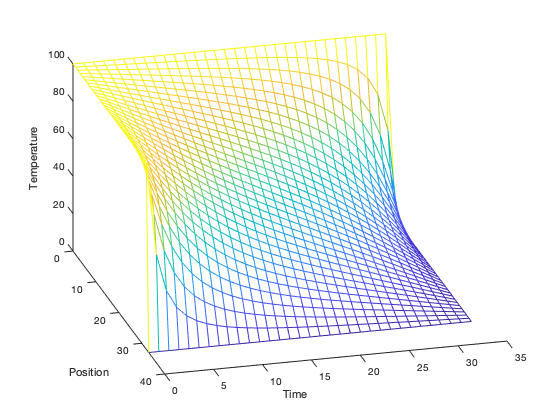
\includegraphics[width=\textwidth]{problem1_1.png}
\label{fig:time1}
\end{subfigure}\hfill
\begin{subfigure}{0.49\columnwidth}
\centering
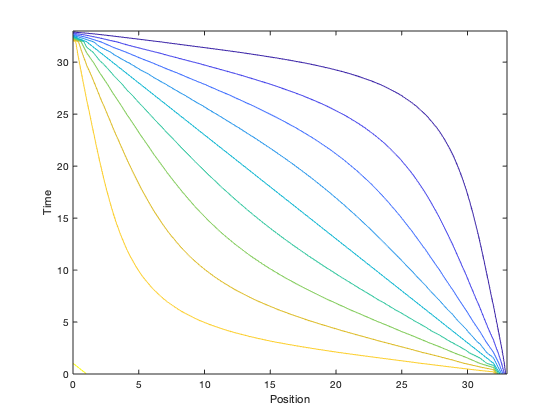
\includegraphics[width=\textwidth]{problem1_2.png}
\end{subfigure}
\caption{(a) A system of a 1D plate that is cooling down (b) contour plot}
\end{figure}

\subsection*{Problem 1b}

The color of the contour plot is the 3rd dimension in this 2D plot. The brighter the color such as the yellow represents the hottest part of the system. While the darker color such as the purple represents the coolest part of the system. If we looked at Figure 1 (a), just the x and y coordinates, then it is the curves we see lay on the grid. What the plot is telling us is that each line is a different temperature ans each line is in a different time and position section. For example the first (lightest yellow) line in the plot has a position range from 10 to 33 given a range of time from 0 to 5. Given the same position range, every other line has a different time range. Therefore, each line tells us the temperature at every point on the 1D line given a time.

\subsection*{Problem 1c}

\begin{figure}[h!]
\centering

\begin{subfigure}{0.49\columnwidth}
\centering
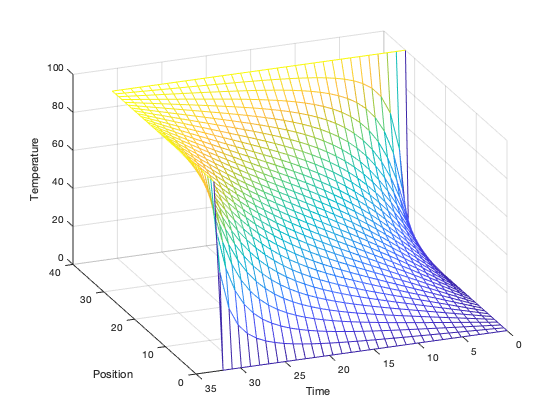
\includegraphics[width=\textwidth]{problem1_3.png}
\label{fig:time1}
\end{subfigure}\hfill
\begin{subfigure}{0.49\columnwidth}
\centering
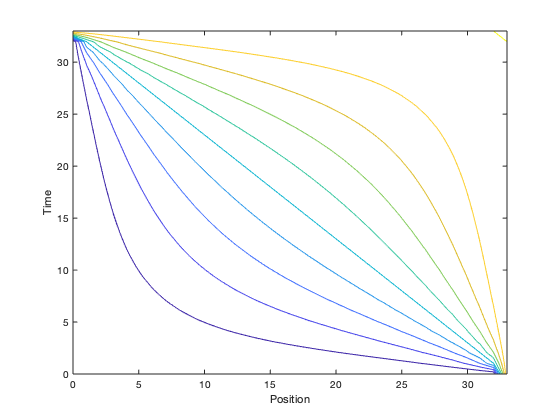
\includegraphics[width=\textwidth]{problem1_4.png}
\end{subfigure}
\caption{(a) A system of a 1D plate that is heating up (b) contour plot}
\end{figure}

\clearpage

\section*{Problem 2}

\begin{figure}[h!]
\centering

\begin{subfigure}{0.49\columnwidth}
\centering
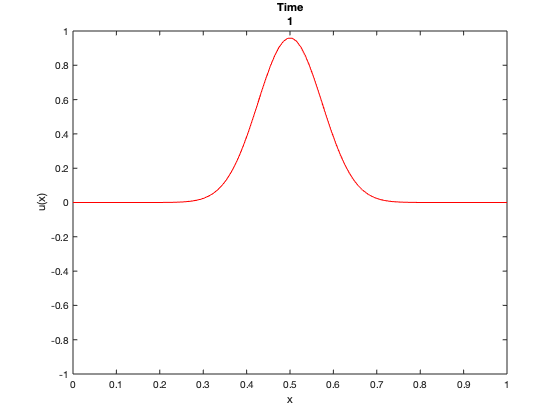
\includegraphics[width=\textwidth]{problem_2_t_1.png}
\caption{}
\label{fig:time1}
\end{subfigure}\hfill
\begin{subfigure}{0.49\columnwidth}
\centering
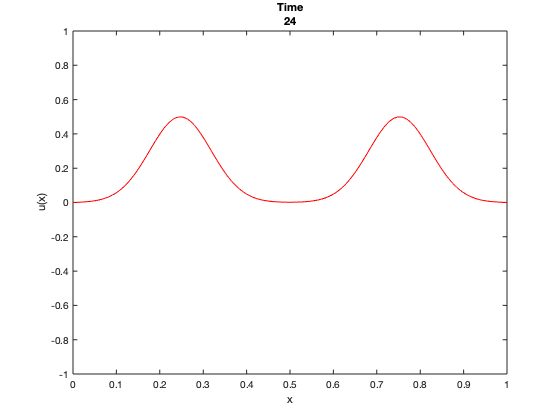
\includegraphics[width=\textwidth]{problem_2_t_24.png}
\caption{}
\label{fig:time2}
\end{subfigure}

\medskip

\begin{subfigure}{0.49\columnwidth}
\centering
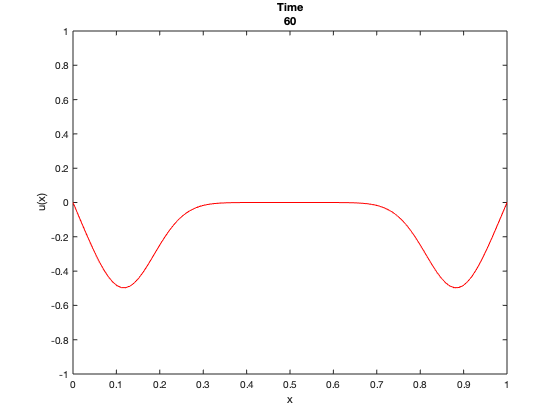
\includegraphics[width=\textwidth]{problem_2_t_60.png}
\caption{}
\label{fig:time3}
\end{subfigure}\hfill
\begin{subfigure}{0.49\columnwidth}
\centering
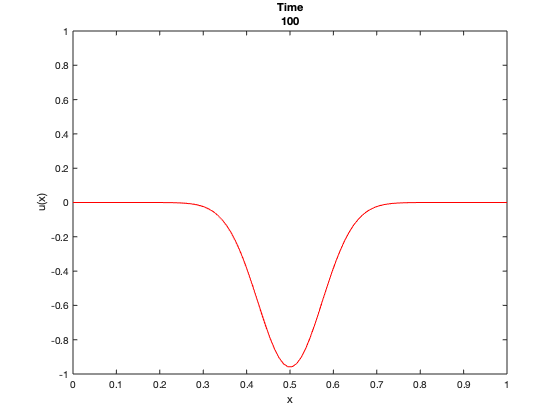
\includegraphics[width=\textwidth]{problem_2_t_100.png}
\caption{}
\label{fig:time4}
\end{subfigure}

\caption{(a) Snapshot at $t = 1$ (b) snapshot at $t = 24$ (c) snapshot at $t = 60$ (d) snapshot at $t = 100$.}
\label{fig:time}

\end{figure}


The plot starts as a Gaussian and then splits into two separate Gaussian waves. One of the Gaussian waves moves to the left while the other moves to the right. When they hit the boundaries they invert and start moving back towards $x = L/2$ and recombine to one Gaussian wave.

\clearpage

\section*{Problem 3}

\begin{figure}[h!]
\centering

\begin{subfigure}{0.49\columnwidth}
\centering
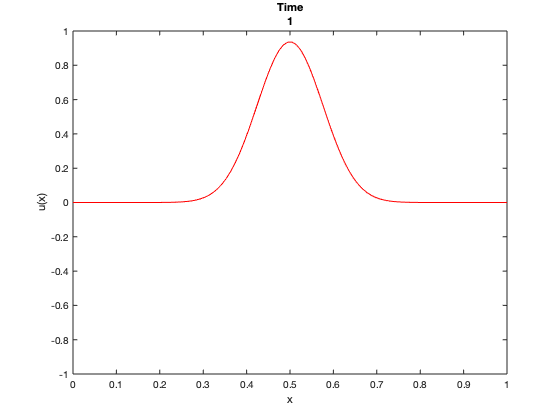
\includegraphics[width=\textwidth]{problem_3_t_1.png}
\caption{}
\label{fig:time1}
\end{subfigure}\hfill
\begin{subfigure}{0.49\columnwidth}
\centering
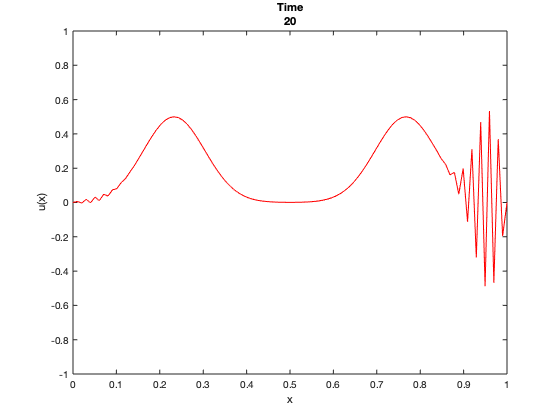
\includegraphics[width=\textwidth]{problem_3_t_20.png}
\caption{}
\label{fig:time2}
\end{subfigure}

\medskip

\begin{subfigure}{0.49\columnwidth}
\centering
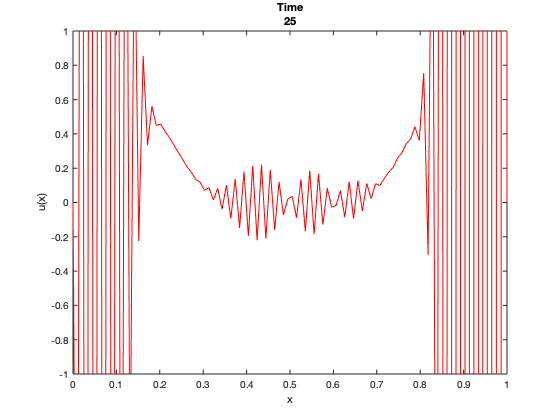
\includegraphics[width=\textwidth]{problem_3_t_25.png}
\caption{}
\label{fig:time3}
\end{subfigure}\hfill
\begin{subfigure}{0.49\columnwidth}
\centering
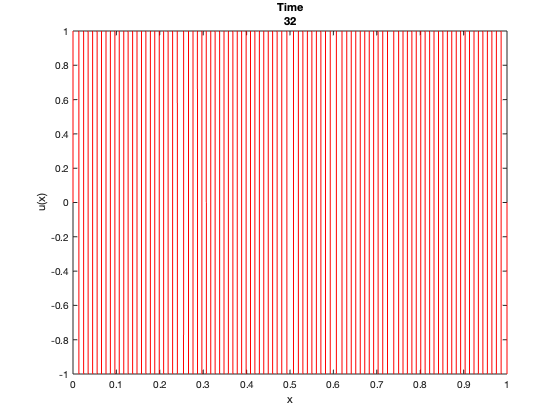
\includegraphics[width=\textwidth]{problem_3_t_32.png}
\caption{}
\label{fig:time4}
\end{subfigure}

\caption{(a) Snapshot at $t = 1$ (b) snapshot at $t = 20$ (c) snapshot at $t = 25$ (d) snapshot at $t = 32$.}
\label{fig:time}

\end{figure}

Picking a value of $\lambda$ such that $\lambda > 1$ produces a numerical error. At $t = 1$ the function looks normal and nothing is wrong with the PDE as of this time. As time increases to around $t = 20$ the first sign of a numerical error occurs on the right side of the plot. Shortly after at $t = 25$ this error increases significantly and becomes even more unstable. The plot at this point is almost completely unrecognizable when looking back at the original solution. The final plot at $t = 32$, the function is completely unstable and completely unrecognizable. It should be noted how fast this unsuitability had occurred and will break even faster the larger $\lambda$ becomes.


\clearpage

\section*{Problem 4}

\begin{figure}[h!]
\centering

\begin{subfigure}{0.49\columnwidth}
\centering
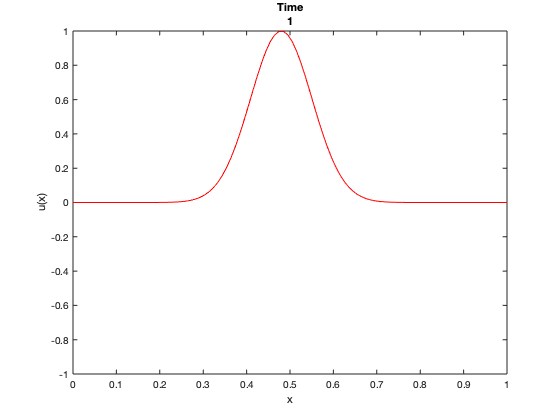
\includegraphics[width=\textwidth]{problem_4_t_1.png}
\label{fig:time1}
\end{subfigure}\hfill
\begin{subfigure}{0.49\columnwidth}
\centering
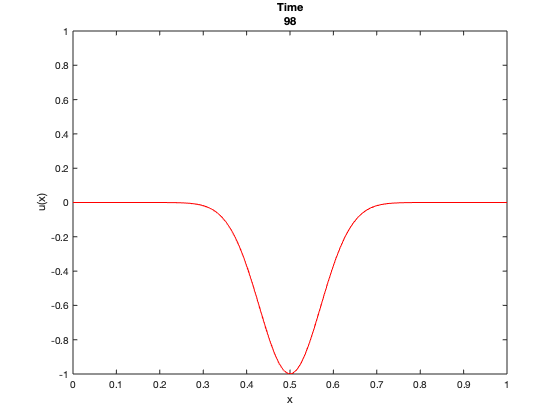
\includegraphics[width=\textwidth]{problem_4_t_98.png}
\end{subfigure}
\caption{Snapshot at $t = 1$ (b) snapshot at $t = 20$}
\end{figure}

The wave no longer splits when the following is implemented

$$
u_{t}(t = 0) = -200x(x - 0.5)e^{-100(x + ct - 0.5)^2}
$$.

Instead the wave remains a single wave and moves to the left until it hits $x = 0$. Then the wave inverts and moves to the right until $x = L$, when it inverts again. These steps will continue to repeat till $t = tf$, where $tf$ is final time.

\clearpage

\section*{Problem 5}

\begin{figure}[h!]
\centering

\begin{subfigure}{0.49\columnwidth}
\centering
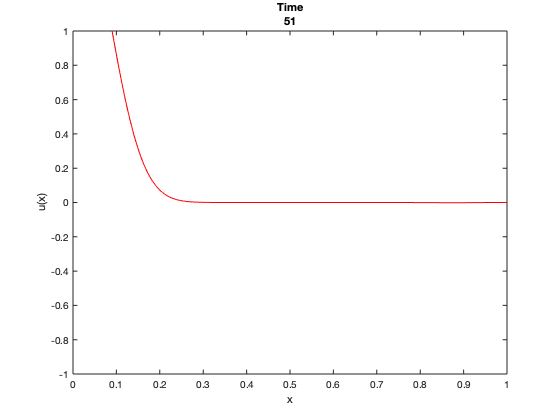
\includegraphics[width=\textwidth]{problem_5_1.png}
\label{fig:time1}
\end{subfigure}\hfill
\begin{subfigure}{0.49\columnwidth}
\centering
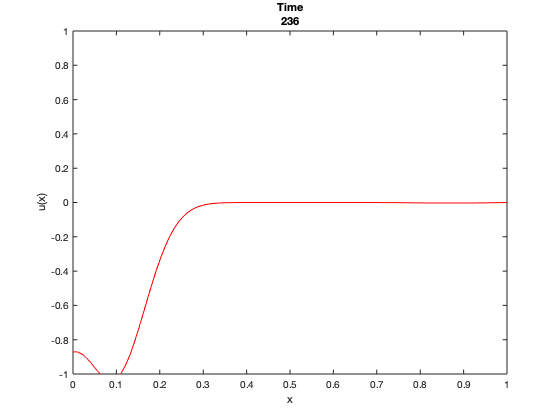
\includegraphics[width=\textwidth]{problem_5_2.png}
\end{subfigure}
\caption{(a) Snapshot at $t = 51$ shows no constraint at $x = 0$ (b) Snapshot at $t = 236$ shows no constraint at $x = 0$ when the Gaussian is inverted}
\end{figure}

After setting $u(1) = u(2)$ there is no longer a constraint at $x = 0$ and the wave allows for $u(0, t)$ to update. From this, the results are shown in Figure 6.


\begin{figure}[h!]
\centering
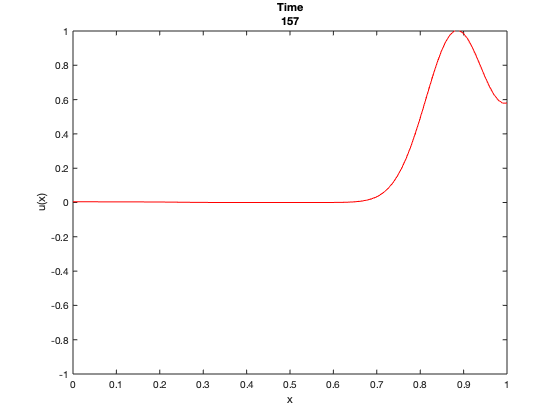
\includegraphics[width=\textwidth]{problem_5_3.png}
\caption{Snapshot at $t = 1$ and $x = L$}
\end{figure}

Figure 7 is an example of if there is no constraint at $x = L$.

\clearpage


\section*{Appendix}

\subsection*{Homework 6 Main Function}
\begin{lstlisting}[language=Matlab, caption= ]
function homework_6()

    fprintf('Enter an integer for what problem you want to run 1-5\n')
    prompt = input('What problem do you want to run? \n problem: ');


    if prompt == 1
        problem_1()

    elseif prompt == 2
        problem_2()

    elseif prompt == 3
        problem_3()

    elseif prompt == 4
        problem_4()

    elseif prompt == 5
        problem_5()

    else
        fprintf("Invalid input")
        
    end

end

function problem_1()

    N = 33;  % Grid size
    maxiter = 1000;
    
    x0 = 0;
    dx = N;
    xf = 33;
    t0 = 0;
    dt = N;
    tf = 33;
    
    x = linspace(x0, xf, N)';
    t = linspace(t0, tf, N)';
    
    u0x = 100;
    ufx = 0;
    u0t = 100;
    uft = 0;

    u = MyHeatEq(N, maxiter, u0t, u0x, uft, ufx);

    hold on
    figure(1)
    [x, t] = meshgrid(x, t);
    surf(x, t, u);
    mesh(x, t, u);
    xlabel('Position');
    ylabel('Time');
    zlabel('Temperature');
    
    hold on
    figure(2)
    contour(x, t, u)
    xlabel('Position');
    ylabel('Time');
    zlabel('Temperature');
    
    fprintf("There is a pause, press any button to continue")
    pause;
    
    u0x = 0;
    ufx = 100;
    u0t = 0;
    uft = 100;
    
    x = linspace(x0, xf, dx)';
    t = linspace(t0, tf, dt)';

    u = MyHeatEq(N, maxiter, u0t, u0x, uft, ufx);
    
    size(u)
    
    hold on
    figure(3)
    [x, t] = meshgrid(x, t);
    surf(x, t, u);
    mesh(x, t, u);
    xlabel('Position');
    ylabel('Time');
    zlabel('Temperature');
    
    hold on
    figure(4)
    contour(x, t, u)
    xlabel('Position');
    ylabel('Time');
    zlabel('Temperature');
    
end

function problem_2()

    tau      = 10;     % N Tension
    m        = 0.001;  % kg mass
    x0       = 0;      % x init
    xl       = 1;      % m
    x_length = (xl - x0);
    maxtime  = 20;     % 20time steps
    hx       = 0.01;   % cm
    dt       = 0.0001; % s
    
    N      = round(x_length/hx);
    x      = linspace(x0, xl, N);
   
    du0    = zeros(1, N);
    
    u  = exp(-100 * (x - 0.5).^(2));
    u0 = u;
    
    %u0(1)  = 0.0; 
    u0(N)  = 0.0; 
    
    mu =  m/x_length; % m density 
    c = sqrt(tau/mu); %tau/m

    MyString(c, x, x_length, u, u0, du0, N, maxtime, hx, dt)

end

function problem_3()

    tau      = 25;     % N Tension
    m        = 0.001;  % kg mass
    x0       = 0;      % x init
    xl       = 1;      % m
    x_length = (xl - x0);
    maxtime  = 20;     % 20time steps
    hx       = 0.01;   % cm
    dt       = 0.0001; % s
    
    N      = round(x_length/hx);
    x      = linspace(x0, xl, N);
   
    du0    = zeros(1, N);
    
    u  = exp(-100 * (x - 0.5).^(2));
    u0 = u;
    
    %u0(1)  = 0.0; 
    u0(N)  = 0.0; 
    
    mu =  m/x_length; % m density 
    c = sqrt(tau/mu); %tau/m

    MyString(c, x, x_length, u, u0, du0, N, maxtime, hx, dt)

end

function problem_4()

    tau      = 10;     % N Tension
    m        = 0.001;  % kg mass
    x0       = 0;      % x init
    xl       = 1;      % m
    x_length = (xl - x0);
    maxtime  = 20;     % 20time steps
    hx       = 0.01;   % cm
    dt       = 0.0001; % s
    
    N = round(x_length/hx);
    x = linspace(x0, xl, N);
    
    mu =  m/x_length; % m density 
    c = sqrt(tau/mu); %tau/m
    
    t   = 0;
    u   = exp(-100 * (x + (c * t) - 0.5).^(2));
    u0  = u;
    du0 = -200 * c * (x - 0.5).*exp(-100 * (x + (c * t) - 0.5).^2); 
    
    %u0(1)  = 0.0; 
    u0(1)  = 0.0; 
    du0(1) = 0;
    u0(N)  = 0.0; 

    MyString(c, x, x_length, u, u0, du0, N, maxtime, hx, dt)

end

function problem_5()

    tau      = 10;     % N Tension
    m        = 0.001;  % kg mass
    x0       = 0;      % x init
    xl       = 1;      % m
    x_length = (xl - x0);
    maxtime  = 20;     % 20time steps
    hx       = 0.01;   % cm
    dt       = 0.0001; % s
    
    N = round(x_length/hx);
    x = linspace(x0, xl, N);
    
    mu =  m/x_length; % m density 
    c = sqrt(tau/mu); %tau/m
    
    t   = 0;
    u   = exp(-100 * (x + (c * t) - 0.5).^(2));
    u0  = u;
    du0 = -200 * c * (x - 0.5).*exp(-100 * (x + (c * t) - 0.5).^2); 
    
    %u0(1)  = 0.0; 
    u0(1)  = 0.0; 
    du0(1) = 0;
    u0(N)  = 0.0; 
    u0(2)   = u0(3);

    MyString(c, x, x_length, u, u0, du0, N, maxtime, hx, dt)

end














\end{lstlisting}

\subsection*{MyHeatEq.m}
\begin{lstlisting}[language=Matlab, caption= ]
function [u] = MyHeatEq(N, maxiter, u0t, u0x, uft, ufx)

    sqrt_alpha = sqrt(4 - (2*cos(pi/N))^2);
    alpha      = (4/(2 + sqrt_alpha)) - 1;

    tol      = 5.e-5;      
    u        = zeros(2,N); 
    u(1,1:N) = u0t;
    u(1:N,1) = u0x;
    u(N,1:N) = uft;  
    u(1:N,N) = ufx; 
    count    = 0; 
    done     = false; 
    while ~done 
        done  = true;                
        count = count + 1; 
        if (count >= maxiter), error( 'Too many iterations!'); end 
        for i = 2: N-1 
            for j = 2: N-1 
                uu = .25*(u(i+1,j) + u(i-1,j)+u(i,j+1)+u(i,j-1)); 
                if(abs((uu-u(i,j))/uu) > tol), done = false; end 
                u(i,j) = uu + alpha *(uu -u(i,j));  
            end 
        end 
    end 
end
\end{lstlisting}

\subsection*{MyString.m}
\begin{lstlisting}[language=Matlab, caption= ]
function MyString(c, x, x_length, u, u0, du0, N, maxtime, hx, dt)


    epsilon = (dt * c/hx); % Needs to remain < 1 to insure stability 
    % if epsilon > 1 % Courant number
    %     disp(epsilon)
    %     error('epsilon too large, PDE will be unstable')
    % end

    %% Preallocate
    %u     = zeros(1, N);
    %u      = zeros(1, N);
    %u0     = zeros(1, N);

    u_old = u0;
    u_new = zeros(1, N);
    time  = 0.0;  % Init time (t0)

    for i = 2:(N - 1)
        u(i) = 0.5 * epsilon * (u0(i + 1) + u0(i - 1)) + ... 
               (1.0 - epsilon) * u0(i) + dt * du0(i); 
    end 

    %% Start main time loop 
    tdisp = 0;
    fig = figure;

    while time < maxtime 
        if ~ishghandle(fig)
            break
        end

        time  = time + dt;
        tdisp = tdisp + 1;

        for i = 2:(N - 1) 
            u_new(i) = epsilon * (u(i + 1) + u(i - 1)) + ... 
                      2.d0 * (1.0 - epsilon) * u(i) - u_old(i);
        end 

        u_old = u; 
        u     = u_new; 

        %% plot
        pause(0.01)

        plot(x, u, 'r');
        axis([0 x_length -1 1]);
        title(["Time", tdisp])
        xlabel("x")
        ylabel("u(x)")

    end
    close(fig);

end
\end{lstlisting}


%\subsection*{line Fit}
%\begin{lstlisting}[language=Matlab, caption= ]
%
%\end{lstlisting}

% --------------------------------------------------------------
%                           End Document.
% --------------------------------------------------------------
 
\end{document}

